\documentclass[aps,prd,preprint,nofootinbib]{revtex4-2}
\usepackage{amsmath,amssymb,bm,booktabs,graphicx,microtype}
\usepackage[hidelinks]{hyperref}

\begin{document}

\title{Lag-Conditioned Recovery of Two Rotation Rates from a Palindromic Recurrence}
\author{Meridian Calder}
\affiliation{SAT/H(s)H Sandbox Geometry Program}
\date{27 September 2026}

\begin{abstract}
A trajectory generated by two independent planar rotation rates obeys an exact
fourth-order palindromic recurrence.  We derive the exact cosine-root
discriminant as a function of sampling lag and show that adjacent-sample
recovery is intrinsically driven toward a fourth-order discriminant collapse.
A fixed, answer-blind lag rule is then tested numerically on a controlled
four-coordinate double-rotation signal.  Under the declared acquisition and
noise configuration, the same structured least-squares estimator that is
poorly conditioned at short lag recovers a frequency gap of $0.10$ with
sub-percent median relative error at the selected stride, while substantially
smaller gaps cross the observed resolution frontier.  The result is a
mathematical and numerical identifiability statement for this signal model,
not a claim about physical dynamics.
\end{abstract}

\maketitle

\section{Model and recurrence}

Consider
\begin{equation}
\bm x(t)=
\left(
a\cos\omega t,\,
a\sin\omega t,\,
b\cos\nu t,\,
b\sin\nu t
\right).
\end{equation}
Sampling at a lag $\tau=L\Delta t$ gives characteristic roots
$e^{\pm i\omega\tau}$ and $e^{\pm i\nu\tau}$.
Each coordinate therefore obeys
\begin{equation}
c_{n+4L}-s_1c_{n+3L}+s_2c_{n+2L}
-s_1c_{n+L}+c_n=0,
\label{eq:recurrence}
\end{equation}
where
\begin{align}
s_1&=2\left[\cos(\omega\tau)+\cos(\nu\tau)\right],\\
s_2&=2+4\cos(\omega\tau)\cos(\nu\tau).
\end{align}
The two cosine modes are roots of
\begin{equation}
q^2-\frac{s_1}2q+\frac{s_2-2}4=0.
\end{equation}

\section{Lag-conditioned discriminant}

The quadratic discriminant reduces exactly to
\begin{align}
\Delta_q(\tau)
&=
\left[\cos(\omega\tau)-\cos(\nu\tau)\right]^2\\
&=
4\sin^2\!\left[\frac{(\omega+\nu)\tau}2\right]
 \sin^2\!\left[\frac{(\omega-\nu)\tau}2\right].
\label{eq:disc}
\end{align}
Consequently,
\begin{equation}
\Delta_q(\tau)
=
\frac{(\omega^2-\nu^2)^2}4\,\tau^4
+O(\tau^6)
\end{equation}
as $\tau\rightarrow0$.
Thus exact recurrence validity does not imply stable adjacent-sample
identifiability.  The same expression also identifies collision lags at which
either sine factor vanishes; ``use the largest possible lag'' is therefore
not an invariant prescription.

\section{Controlled numerical benchmark}

We used $a=1.2$, $b=0.65$, $\omega=1.1$, $\Delta t=0.025$,
161 samples over $[-2,2]$, and independent coordinate noise
$\mathcal N(0,10^{-8})$.  At each stride, a single pair $(s_1,s_2)$ was
estimated by ordinary least squares from all four coordinates under the
palindromic structure of Eq.~(\ref{eq:recurrence}).  No total-least-squares
claim is made.

The declared target gap set was
$\Delta\omega\in\{0.10,0.03,0.01,0.003\}$.
Before examining recovery error, the stride was selected by
\begin{equation}
L_\star=
\arg\max_L
\min_{\Delta\omega}
\Delta_q(L\Delta t),
\end{equation}
subject to retaining at least 40 recurrence windows.  This gives
$L_\star=30$.

\begin{table}[b]
\caption{Deterministic-seed noisy benchmark at the answer-blind selected stride.
Errors are relative to the true frequency gap; 120 trials were used per row.}
\centering
\begin{ruledtabular}
\begin{tabular}{ccc}
$\Delta\omega$ & median relative error & 95th percentile\\
\hline
0.10  & 0.00690 & 0.02448\\
0.03  & 0.09252 & 0.23562\\
0.01  & 0.52350 & 1.43447\\
0.003 & 33.54698 & 48.21774\\
\end{tabular}
\end{ruledtabular}
\end{table}

\begin{figure}
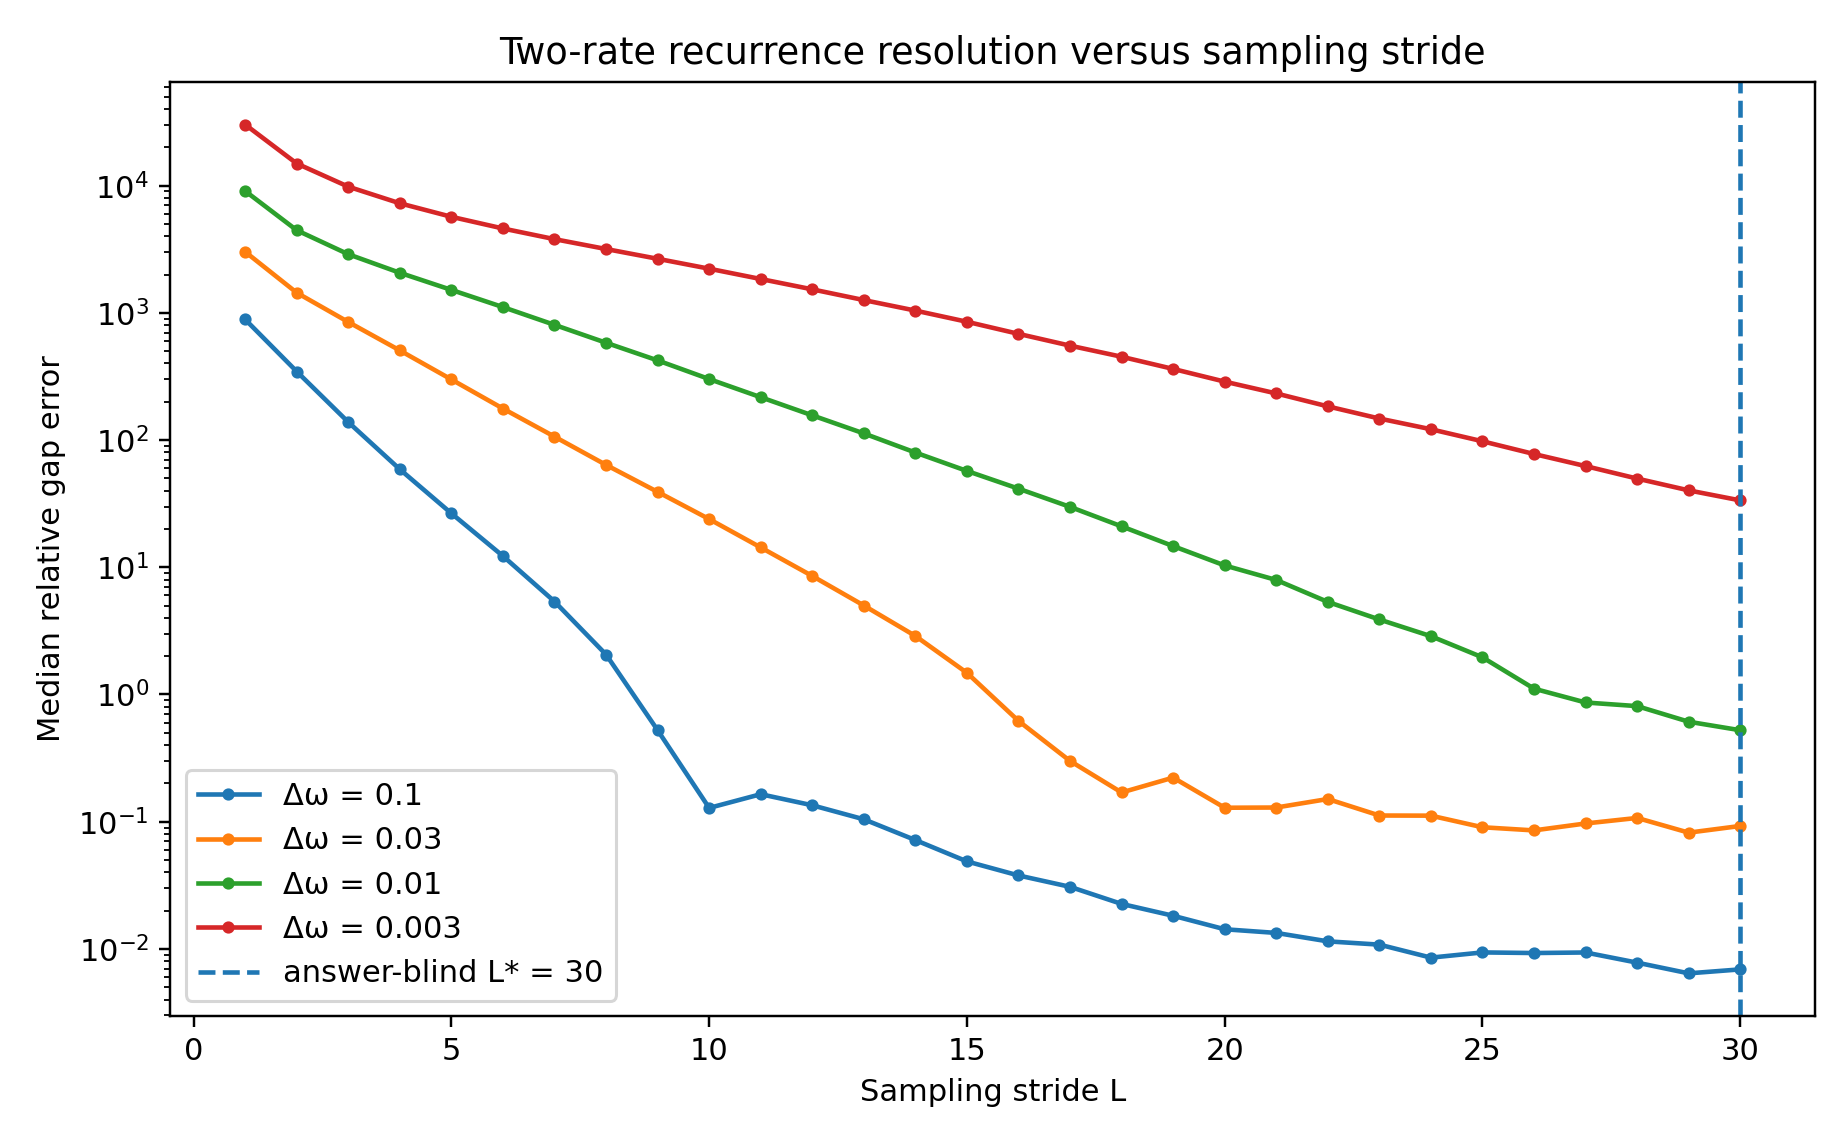
\includegraphics[width=\columnwidth]{recurrence_resolution_frontier.png}
\caption{Median relative gap-recovery error versus sampling stride.
The vertical marker is the answer-blind stride selected from the exact
discriminant rather than from observed recovery error.}
\end{figure}

\section{Use and limits}

For the SAT/H(s)H sandbox, Eq.~(\ref{eq:disc}) supplies a controlled
front end for reconstructing paired rotation rates before any proposed
translation into frame-history or the Hagalaz transform machinery.
Outside that context, the same derivation is a generic identifiability result
for any sampled two-frequency signal with the palindromic characteristic
polynomial above.

The numerical frontier is not universal: it depends on duration, cadence,
noise, amplitudes, estimator, and alias constraints.  What survives those
choices is the exact recurrence and its lag-dependent discriminant.

\end{document}
